%%%%%%%%%%%%%%%%%%%%% chapter.tex %%%%%%%%%%%%%%%%%%%%%%%%%%%%%%%%%
%
% sample chapter
%
% Use this file as a template for your own input.
%
%%%%%%%%%%%%%%%%%%%%%%%% Springer-Verlag %%%%%%%%%%%%%%%%%%%%%%%%%%
%\motto{Use the template \emph{chapter.tex} to style the various elements of your chapter content.}

\chapter{Meshbased Methods} % Main chapter title

\label{Chapter4} % Change X to a consecutive number; for referencing this chapter elsewhere, use \ref{ChapterX}


%----------------------------------------------------------------------------------------
%	SECTION 1
%----------------------------------------------------------------------------------------

\section{Meshbased discrectization}

In this chapter the three most important meshbased discretization methods are introduced and explained in great detail. For further reading on these methods
Ferziger2002 provides a excellent overview. 


\section{FDM}

The Finite Difference Method (FDM) is the easiest and and oldest discretization method. The occuring partial derivatives in the CFD equations
are replaced or better approximated by algebraic finite difference quotients. The approximations of the derivatives rest on Taylor series
expansions and the method will be explained with a simple example before moving to 
the NSE equations. For further, extensive reading on FDM chap. 8 Pozrikidis2009 is recommended.

\subsection{Basic Idea of FDM}

Given a function $ f(x) $ the derivative $\partial f$  at a certain point x can be defined by


\begin{equation} \label{eq:fdm_con}
\frac {\partial f}{\partial x}  = 
\lim_{h \to 0} \frac {f(x+h)-f(x)}{h} 
\end{equation}

Now to bring this function into a finite and computable space, the limit is replaced by a sufficiently small and finite $h$:

\begin{equation} \label{eq:fdm_con_to_desc}
\frac {\partial f}{\partial x}  \approx
\frac {f(x+h)-f(x)}{h} 
\end{equation}

The continuous function \ref{eq:fdm_con} has now been discretized to the approximation
\ref{eq:fdm_con_to_desc}.  By multiplying this equation with $h$ on both sides and solving it to $f(x+h)$ we now receive:

\begin{equation} \label{eq:fdm_eulerform}
f(x+h) \approx
f(x) + \frac {\partial f}{\partial x} h
\end{equation}

In this form the left hand side (LHS) represents a the value of the function itself
at a point $(x+h)$ and this value can be approximated by the term on the right hand side (RHS). This  simple form \ref{eq:fdm_eulerform}
of discretization is called \emph{Euler's Method}. It is the simplest Taylor Series expansion (TSE) of a function when only the first
Taylor polynomial in the expansion is used. Thus FDM is heavily based on TSE and in order to better understand the types and magnitude of errors that occur by discretizing
a function with finite differences the following section will discuss the Taylor series analysis of FDM.

\subsection{Taylor series expansion and error analysis}
\label{sec:taylor_ser_num_ana}

The exact TSE of the above function $ f(x) $ when developing it around $x$ with the step $h$ is:

\begin{equation} \label{eq:fdm_tse_full}
f(x+h) =
\sum_{i=0}^{\infty}\frac{\partial^i f}{\partial x^i} \frac {h^i}{i!} = 
f(x) + \frac {\partial f}{\partial x} h + \frac {\partial^2 f}{\partial x^2} \frac {h^2}{2!} + \frac {\partial^3 f}{\partial x^3} \frac {h^3}{3!} + ...
\end{equation}

The RHS of the equation \ref{eq:fdm_tse_full} is again a continuous and exact description of the function itself. Even for very large arbitrary values of $h$ this description
would give a exact solution at  the point $x+h$.  In order to discretize and gain a finite amount of terms on the RHS that can be evaluated by a computer, the infinite
series needs to be truncated. The type of error that this truncation introduces is called \textbf{truncation error}:

\begin{equation}
f(x+h) =
\underbrace{f(x) + \frac {\partial f}{\partial x} h}_{Approximation} + 
\overbrace{\frac {\partial^2 f}{\partial x^2} \frac {h^2}{2!} + \frac {\partial^3 f}{\partial x^3} \frac {h^3}{3!} + ...}^{Truncation\ error}
\end{equation}

This notation can be rearranged to better understand the meaning of the Truncation error:


\begin{equation}\label{eq:fdm_vs_trunc}
\overbrace{\frac {f(x+h) - f(x)}{h}}^{finite\ difference} - 
\underbrace{\frac{\partial f}{\partial x}}_{derivative} =
\overbrace{\frac {\partial^2 f}{\partial x^2} \frac {h}{2!} + \frac {\partial^3 f}{\partial x^3} \frac {h^2}{3!} + ...}^{Truncation\ error}
\end{equation}

The truncation error in equation \ref{eq:fdm_vs_trunc} can now be better understood as the difference between the discretized finite difference and the actual continuous derivative. Before moving on the actual grids, one needs to understand the important relationship between the grid spacing $h$ and the 
truncation error which can be denoted with the Landau notation. As it will be shown in the following part, the truncation error is a strong indicator of how fast the error of a finite difference approximation decreases when the grid spacing $h$ is decreasing.

Rewriting equation \ref{eq:fdm_vs_trunc} and solving it for the finite difference
shows:

\begin{equation}\label{eq:fdm_vs_fd}
\frac {f(x+h) - f(x)}{h} = 
\frac{\partial f}{\partial x} + 
\frac {\partial^2 f}{\partial x^2} \frac {h}{2!} + \frac {\partial^3 f}{\partial x^3} \frac {h^2}{3!} + ...
\end{equation}

Under the assumption that $h \leq 1 $ the truncation error in equation \ref{eq:fdm_vs_fd} can be reduced to its most dominant term which is of linear nature. This leads to the Big - $\mathcal{O}$ notation which denotes that the truncation error is proportional to the  the grid spacing $h$.

\begin{equation}\label{eq:fdm_vs_linod}
\frac {f(x+h) - f(x)}{h} \cong
\frac{\partial f}{\partial x} + 
\frac {\partial^2 f}{\partial x^2} \frac {h}{2!} = 
\frac{\partial f}{\partial x} + \mathcal{O}(h)
\end{equation}

When focusing on the most LHS and RHS of equation \ref{eq:fdm_vs_linod} the connection between the FDM approximation in equation \ref{eq:fdm_con_to_desc}
and the error analysis lead to the observation, that this approximation and its error is proportional and therefore of \emph{first order}. At the beginning of this section the equation \ref{eq:fdm_con} used a one-sided step $x+h$ forward in the general description of the derivative. Therefore this difference formula is called \emph{one-sided forward difference of first order}.

The same technique can be used for a backward difference with the step $x-h$. But this will also only lead to a first order difference. Both of these one sided, single step methods are as already stated know as \emph{Euler's Method} and are usually not used in high efficient engineering CFD implementations. To achieve a faster truncation error approach to zero when decreasing the grid spacing $h$ multiple steps have to be made and combined. A simple example of this is the central difference method that adds up the forward difference and the backward difference and hence has a accumulated step of $2h$. This leads to a second order
approximation:

\begin{equation}\label{eq:fdm_centraldiff}
\frac {f(x+h) - f(x-h)}{2h} = 
\frac{\partial f}{\partial x} + \mathcal{O}(h^2)
\end{equation}

In the following section the implications of the first and second order methods concering the mesh itself are illustrated. Above Euler's Method and the central difference method, there are many other multi step methods that are used today. For further reading please refer to Milne2000.


\subsection{Structured Meshes in FDM}

\subsection{Problems of FDM}
\label{sec:problems_of_fdm}
\subsubsection{Problems with conservation}
\subsubsection{Problems with irregular meshes}



\section{FVM}

The Finite Volume Method (FVM) is the standard discretization and solving method for 
CFD. It is based on the concept of conservative discretization, which will be discussed in this chapter. In contrast to the previous discussed FDM which used the differential form of a equation for discretization, the FVM uses the \emph{integral} form of such. And transfers volume descriptions into surface integral descriptions with the divergence theorem. As will be shown in this Chapter this method is far superior and more intutive for applications like CFD since its approximations inherently satisfy the conservation conditions of equations which leads it to be much more robust when it comes to complex unstructured meshes and deformations. Above that using the integral form makes the usage of Neumann boundary conditions much easier. For further reading please refer to Leveque2002.


\subsection{Basic Idea of FVM}
The simplest and most striking fact of the NSE is that most of the equations are used to \textbf{conserve} some quantity like momentum, mass or energy. To simulate a fluid flow these conservation equations need to be solved. The name FMV is based on the idea that a domain is subdivided into a finite amount of volumes. To start diving into the integral descriptions of FVM, first consider $ \kappa $ to be a arbitrary density of a conservative quantity and $\Omega$ a certain control volume in $R^3$.   

To describe the total amount of $\kappa$ inside $\Omega$ it can be written in integral form as:

\begin{equation}\label{eq:fvm_amountsumkappa}
\int\limits_{\Omega} \kappa d \Omega
\end{equation}



When $\Omega$ moves through space, it not only changes its location but in might also change its shape dependend on time $t$. Therefore if we want to denote a overall change of the quantity $\kappa$ inside of $\Omega$ ,  equation \ref{eq:fvm_amountsumkappa} needs to be changed to:

\begin{equation}\label{eq:fvm_amountsumkappa_deptime}
\frac {d}{dt} \int\limits_{\Omega (t)} \kappa d \Omega
\end{equation}

Within the control volume $\Omega$, a \textbf{conservative} quantity $\kappa$  neighter gets destroyed (sink) nor created (source). Hence the total amount of 
$\kappa$ within $\Omega$ can only change by the \emph{flux} in and out of the volume boundaries of $\Omega$. Let the RHS be a generalized change in flux:

\begin{equation}\label{eq:fvm_amountsumkappa_deptime_flux}
\frac {d}{dt} \int\limits_{\Omega (t)} \kappa d \Omega = RHS
\end{equation}

When the shape of $\Omega$ changes over time, this results in the boundaries in  $(x, y, z)$ beeing time dependent. By decomposing the LHS of \ref{eq:fvm_amountsumkappa_deptime_flux} with the Leibniz parameter integral rules into the boundaries we get:

% \begin{equation}\label{eq:fvm_amountsumkappa_deptime_decomp}
% \begin{split}
% \frac {d}{dt} \int\limits_{\Omega (t)} \kappa d \Omega &=
% \frac {d}{dt} \int\limits_{x_{0}(t)}^{x_{1}(t)} \int\limits_{y_{0}(t)}^{y_{1}(t)} \int\limits_{z_{0}(t)}^{z_{1}(t)} \kappa d \Omega \\ &= 
% \int\limits_{\Omega (t)} \frac{\partial \kappa}{\partial t} d \Omega  + 
% \biggl [\int\limits_{A_{x}(t)} \Bigl ( \kappa \frac{\partial x}{\partial t} \Bigr) d A_{x} \biggr]_{x_{0}(t)}^{x_{1}(t)}    \\ &+ 
% \biggl [\int\limits_{A_{y}(t)} \Bigl ( \kappa \frac{\partial y}{\partial t} \Bigr) d A_{y} \biggr]_{y_{0}(t)}^{y_{1}(t)}   +
% \biggl [\int\limits_{A_{z}(t)} \Bigl ( \kappa \frac{\partial z}{\partial t} \Bigr) d A_{z} \biggr]_{z_{0}(t)}^{z_{1}(t)}
% \end{split}
% \end{equation}

Where $A$ denotes the area of the volume in one dimension. Because all the spatial partial derivatives (x, y, z) are derived by time, they can be considered to be the velocity components $u_{x}, u_{y}, u_{z}$ of the volume $\Omega$ itself. Rewriting the LHS with the closed surface integral notation leads to:

\begin{equation}\label{eq:fvm_amountsumkappa_deptime_oint}
\frac {d}{dt} \int\limits_{\Omega (t)} \kappa d \Omega = 
\int\limits_{\Omega (t)} \frac{\partial \kappa}{\partial t} d \Omega  + 
\oint\limits_{A(t)} \kappa \bar{u} d \bar{A}   
\end{equation}

Thereby $\bar{A}$ denotes the entire closed surface of the volume $\Omega$ and the vector
$\bar{u}$ denotes the velocity of the volume. This equation is a form of Reynolds 
transport theorem and of utterly importance to the conservation idea in FVM, for further explanation please refer to pg. 10 Wesseling2009.
Using the divergence theorem equation \ref{eq:fvm_amountsumkappa_deptime_oint} with the RHS from \ref{eq:fvm_amountsumkappa_deptime_flux} 
the equation can be formulated to a integral form:

\begin{equation}\label{eq:fvm_cons_form_conservat}
\frac {d}{dt} \int \kappa d \Omega = 
\int \biggl [\frac{\partial \kappa}{\partial t} + \nabla \cdot \kappa \bar{u} \biggr] d \Omega = RHS
\end{equation}


\subsubsection{Conservative property}

%- The domain is subdivided into non-overlapping finite control volumes
%- For each control volume only a median value is considered
%- Volume integrals can be tranformed to Surface integreal with divergence theorem
%FVM does not rely on any special mesh structure.

%FVM is cell-averaged values

For further reading please refer to Versteeg2007 and Leveque2002.

\subsection{FVM vs. FDM}

This comparison gives a brief overview of the differences and similarities between
FVM and FDM:
\begin{table}[htp]
\centering
\begin{tabular}{c|c|c}\label{fig:FVM_vs_FDM_simi}
 & FVM & FDM \\
\hline
Conservation laws discretization & Integral form & Differential form \\
\hline
Value type & Cell averaged values & Local function values \\
\end{tabular}
\caption{Comparison of FVM and FDM}
\end{table}





FMV has several advantages over FDM, which are summarized in the follwing list:

\begin{itemize}
\item Flexible spatial discretization
\item The integral form is more intutive than the differential form
\item FVM is closer to the physics of a fluid flow
\end{itemize}

A main disadvantages is that FMV does not have a standardized formal theory to
analyize the accuracy, like FDM uses with Taylor series expansion and analysis.
Still FVM can be "forced" into a structured equidistant mesh which allows a comparative accuracy analysis again FDM.

\section{FEM}
\label{sec:main_fem}
The Finite Element Method (FEM) is usually used in solid and structural mechanics. In contrast to FDM/FVM the Finite Element Method uses also a Lagrangian perspective. Considering Figure \ref{fig:PerspVsDisMeth} FEM is located between the Eulerian
and Langrangian perspective and is Meshbased. It has indeed properties from both
perspectives in his mathematical model. For example in contrast to FDM and FVM, this method uses a \textbf{Lagrangian mesh}, meaning that its mesh is attached to the moving material and moves along with it. Similar to FDM/FVM a division of a continuum into finite domains takes place. These subdivisions of the continuum are called finite discrete elements or simply \emph{elements}. These elements are bound by the mentioned topologial Lagrangian mesh which forbids the penetration or overlapping of similar elements. Each element is used to represent a certain part of the material. During the movement of the mesh, the elements stay associated with their location on the mesh and conserve the properties like mass of themselves.
%ShofanLi S13 Liu2003 p 28
For further reading please refer to Zienkiewicz2005, chap. 10 Wendt2009


%- Difficult to deal with incompressible Fluids ... Zienkiewiczs page 12
%- Difficult to resolve turbulent behaviour -> high resolution grids are required %(Zeinkeiws page 248)
As mentioned previously extremely high mesh resolution is required to obtain
numerical solutions at the smallest turbulence scales. This is very expensive and
presently not possible for high Reynolds number flows. It is, therefore, obvious that
other alternatives are necessary to obtain a viable approximate solution. The current

%Mesh Update problem Zienkiwec 53 an

\subsection{Advantages of FEM}
\label{sec:adv_of_fem}


\subsection{Problems of FEM}
In situations where the solid or fluid undergoes heavy deformation, the mesh and each of its elements will also become highly deformed and distorted. This is very likely to happen, especially in fluids with lower viscosity. Because of this behaviour certain elements can become numerically \emph{inverted}, afterwards representing a negative mass or volume. To avoid this behaviour during a CFD simulation, the mesh needs often needs to undergo the computationally intensive process of remeshing fem. Another way to avoid this is not to use FEM at all and remain with a Eulerian method like FVM. 

\subsubsection{Remeshing}
\label{sec:remeshing_fem}
%Remeshing problem% 228
% \begin{figure}[htp]
% \centering
% 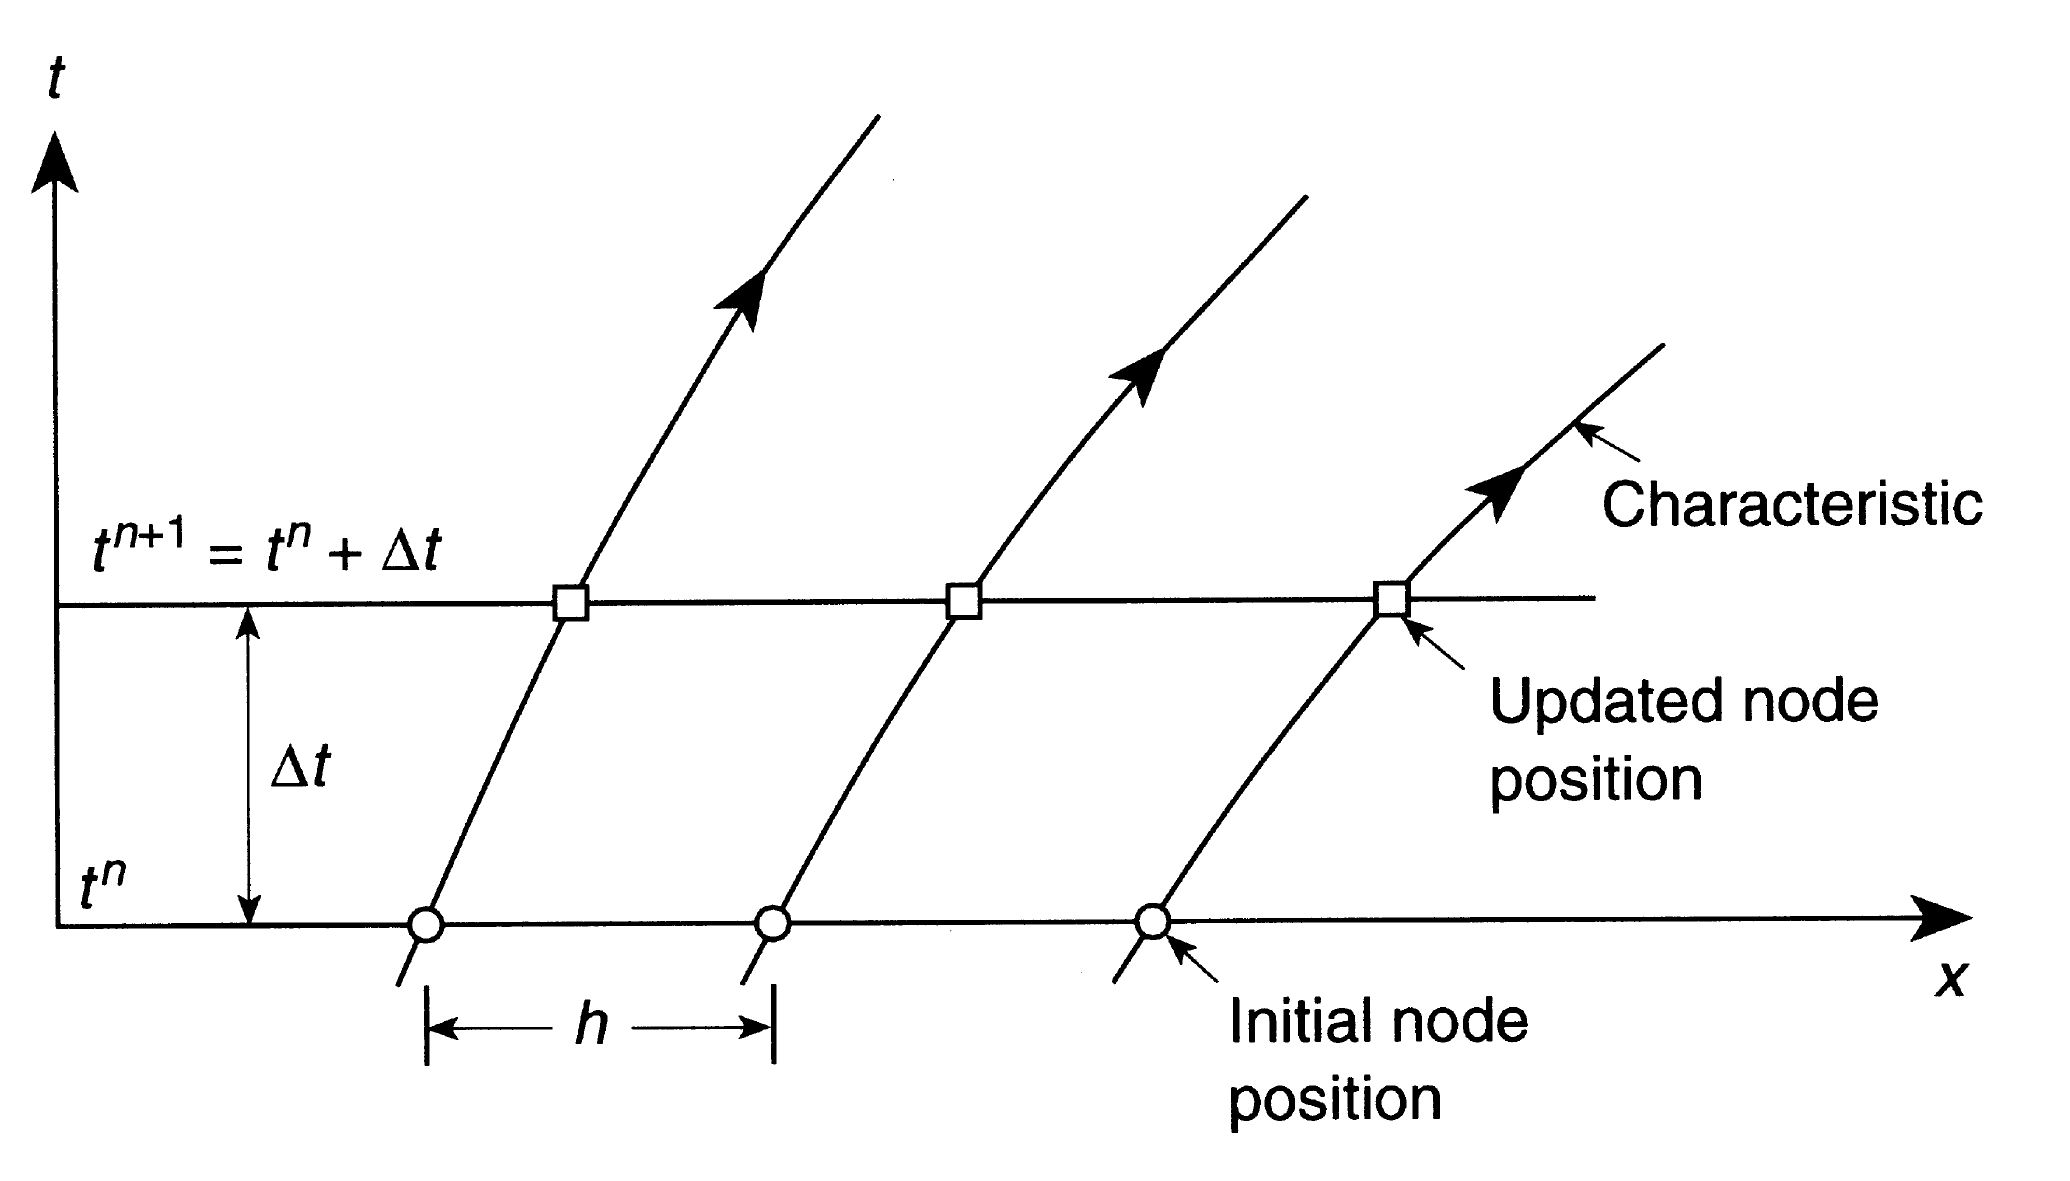
\includegraphics[scale=0.50]{Figures/fem_meshupdate_zienk_53.png}
% \caption{Update of Mesh Nodes in FEM}
% \label{fig:MeshUpdateFEM}
% \end{figure}

\subsubsection{Problems with hyperbolic equations}

\section{Summary of Meshbased Methods}

One clear advantage of FDM and FVM over FEM is the simplicity of the Eulerian mesh.  Because the mesh stays fixed in space, independent from the fluids flow, these methods are also useful for highly deformations. But they come with a high computational costs, since in order to represent these deformations very fine meshes have to be used. This results also in much higher memory consumption that might lead to a limit what kind of fluid problem can be accurately simulated on given hardware. Furthermore FDM and FVM come with a inherently problem of domain communication. In contrast to FEM, both methods need to transport fluid matter from one mesh subdivision to the next during a flow process. This leads to a always necessary numerical communication between neighbouring subdivisions, no matter if a fluid is present in that cell or not. Consequently the domain decomposition on parallel systems leads to a more complicated communications between cluster machines.

%The fluids deformations, both methods do not involve the numerical problems of %Remeshing.

\begin{tabular}{|c|c|c|}
\hline
	Method & Discretization of & @\\
\hline
	FDM & differntial form of conservation equations & @\\
\hline
	FVM & integral form of conservation equations & @\\
\hline
\end{tabular}




